\section{Planning}\label{sec:planning}
The initial schedule for the project can be seen in figure \ref{tab:schedule}. The project will be executed in a scrum-like way.

\begin{figure}[H]
	\begin{center}
		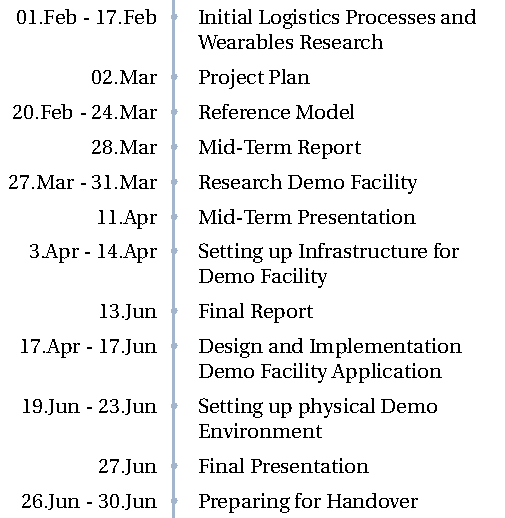
\includegraphics[scale=1]{images/schedule}
	\end{center}
\caption{Schedule}
\label{tab:schedule}
\end{figure}

The schedule is divided in work packages that are to be executed and milestones that are a part of the project. It is to be noted, that each work package could be split into multiple sprints in the future. The milestones are the entries in the schedule that are just having a single date and not a range of dates. In the following subsections the work packages will be explained.

\subsection{Initial Logistics Processes and Wearables Research}
This work package includes research about the given processes and wearables in general, as well as already choosing potential wearables that could be used to improve the process. The end result for this should be a decision on process and wearable. But the result for this could potentially take longer than this task is scheduled. The wearables should be ranked after getting hands-on experience on them, therefore some of them have to be ordered first.

\subsection{Reference Model}
A reference architecture should be created for a sample wearable application. What this work package contains is, the creation of diagrams which show the communication from a wearable to the \gls{wms} or something similar. What should not be created is a full reference architecture for a process that is implemented with a concrete wearable. 

It is about creating the always needed layers when using a wearable in a way that supports most wearable solutions.

\subsection{Research Demo Facility}
This task includes researching what physical objects and what systems would be needed to create a demo facility that could showcase a single process with a single wearable. This also includes the gathering of knowledge of where the demo facility should be created and where to get the needed objects.

\subsection{Setting up Infrastructure for Demo Facility}
The infrastructure for the demo facility includes multiple things, like setting up a server to run a database for the demo facility and creating an interface to connect to it. 

\subsection{Design and Implementation Demo Facility Application}
The work package includes the creation of the software design and implementation for the wearable and further aspects that are needed to fully showcase a process.

\subsection{Setting up physical Demo Environment}
This task includes the physical creation of the demo facility. This means setting up shelves with packages to scan and put on a hand pallet truck. Setting up barcodes on the packages to scan. Setting up an environment that can showcase what is happening better to an audience.

\subsection{Preparing for Handover}
Since this project is part of the bigger logwear research project, the results that were created during this project will be used in the future, therefore all the resources will be made available to a future developer. Furthermore addition documentation and a handover document are part of this work package.